%{{{ Spam
\documentclass[a4paper,12pt]{article}

%use danish hyphenation and titles
%handle utf8-characters
\usepackage[danish]{babel}
\usepackage[utf8]{inputenc}
\usepackage[T1]{fontenc}

%for images
\usepackage[pdftex]{graphicx}

%allow nested figures
\usepackage{subfigure}

%control line spacing
\usepackage{setspace}
%\singlespacing
\onehalfspacing
%\doublespacing

%set margins
%\usepackage[margin=0.75in]{geometry}

%allows margin-notes
%good for work in progress papers
%\usepackage{marginnote}

%allows pretty quoting using ``'' or `'
\usepackage{upquote}

%two definitions of the color grey
\usepackage{color}
\definecolor{listinggray}{gray}{0.9}
%\definecolor{lbcolor}{rgb}{0.9,0.9,0.9}


% References
\usepackage{hyperref}

%allows pretty source code
\usepackage{listings}
\lstset{
  language=,
  literate=
    {æ}{{\ae}}1
    {ø}{{\o}}1
    {å}{{\aa}}1
    {Æ}{{\AE}}1
    {Ø}{{\O}}1
    {Å}{{\AA}}1,
  backgroundcolor=\color{listinggray},
  tabsize=3,
  rulecolor=,
  basicstyle=\scriptsize,
  upquote=true,
  aboveskip={1.5\baselineskip},
  columns=fixed,
  showstringspaces=false,
  extendedchars=true,
  breaklines=true,
  prebreak =\raisebox{0ex}[0ex][0ex]{\ensuremath{\hookleftarrow}},
  frame=single,
  showtabs=false,
  showspaces=false,
  showstringspaces=false,
  identifierstyle=\ttfamily,
  keywordstyle=\color[rgb]{0,0,1},
  commentstyle=\color[rgb]{0.133,0.545,0.133},
  stringstyle=\color[rgb]{0.627,0.126,0.941},
}
%captions on listings
\usepackage[center,font=small,labelfont=bf,textfont=it]{caption}

%allows fancy enumeration
\usepackage{enumerate}

%allows use of the BibTex for the bibliography
\usepackage[numbers]{natbib}

%make references and URLs in the pdf to clickable links
\usepackage{hyperref}

%removes the numbers from sections
\setcounter{secnumdepth}{0}

%proper header formatting
\usepackage{fancyhdr}
\pagestyle{fancy}
\lhead[]{} %clear standard settings
\chead[]{} %clear standard settings
\rhead[]{\rightmark} %current section
\lfoot[]{} %clear standard settings
\cfoot[]{\thepage} %current page number 
\rfoot[]{} %clear standard settings

\usepackage{hyperref} % The package for links. This is also used for the ToC links.
%}}}
\title{\textbf{Heartbeat Protokollen} \\ Bachelorprojekt i Datalogi 2015 - Synopse}
\author{Erik Allin -- smt504 \\ Dennis Olesen -- cwb759}
\date{23. februar 2015}

\begin{document}
\maketitle
\newpage
%\renewcommand*\contentsname{Table of Contents}
%\tableofcontents
%\section*{Forside-lel}
%\newpage
%\clearpage

\section*{Problemformulering}
Er det muligt at konstruere et bibliotek der leverer ressourcehåndtering for et high-availability system med minimalistisk opsætning? 
\\
I hvilken grad kan et sådan system håndtere fejl på de tilsluttede maskiner?

\subsection*{Afgrænsning af problemformulering}
Som udgangspunkt, så er målet med det implementerede program, at det som udgangspunkt skal kunne afvikles på et lokalt netværk.
\\[5px]
Systemet vil som udgangspunkt, fokusere på følgende punkter:
Leader-election, logging samt load-balancing.
\\[5px]
Desuden vil fokus i højere grad ligge på, at holde styr på liveliness og aktivitetsfordeling, end egentligt datahåndtering eller bearbejdning.


\section*{Begrundelse}
Emnet er interessant, da man i forbindelse med udvikling af et distribueret system vil være afhængig af, at kunne sikre sig konsistens og høj tilgængelighed af det involverede system. Metoder til at opdage når en maskine fejler, samt derefter at foretage de nødvendige fejl-procedurer, vil altså være, at finde i størstedelen af de distribuerede systemer.
\\
Ved at konstruere et bibliotek, som gør det simpelt for brugeren at implementere disse metoder vil der både kunne spares udviklingstid for fremtidige projekter, der omhandler distribuerede systemer, og være et fælles produkt at kunne optimere og opdatere, fremfor at skulle tage hensyn til hvert enkelt nye system. Endvidere forventer vi, at man i forbindelse med dette samtidig kan opretholde en balancering af systemernes ressourcer, i forbindelse med de regelmæssige liveliness tjek.
\\[5px]
Et sådant bibliotek vil herved kunne sikre fremtidige applikationer der bruger distribuerede systemer, en fælles og gennemtestet implementation til både load-balancing og liveliness tjek af deres systemer.


\section*{Arbejdsopgaver}

\begin{enumerate}
\item \textbf{Analysere heartbeat-protokollen.} 
\\
\textbf{Produkt}: Analyse-afsnit. \\
\textbf{Ressourcekrav}: Fundet mindst to eksempler på implementationer af heartbeat-protokollen. \\
\textbf{Projekt-interne afhængigheder:} Ingen \\
\textbf{Tidsforbrug:} 4-5 dage \\
\textbf{Deadline:} 26/02-2015
  
\item \textbf{Opstille en API for vores bibliotek.} \\
\textbf{Produkt:} En API for vores produkt, samt en beskrivelse af modulerne. \\
\textbf{Ressourcekrav:} Analyse for system funktionalitet og opsætning. \\
\textbf{Projekt-interne afhængigheder:} Ingen \\
\textbf{Tidsforbrug:} 2-3 dage \\
\textbf{Deadline:} 05/03-2015

\item \textbf{Implementering} \\
\textbf{Produkt:} Vores bibliotek. \\
\textbf{Ressourcekrav:} Vores API, samt bagvedliggende analyse. \\
\textbf{Projekt-interne afhængigheder:} Ingen \\
\textbf{Tidsforbrug:} 15-25 dage \\
\textbf{Deadline:} 19/4-2015

\begin{enumerate}
\item[3.1] \textbf{Connection / Discovery:} \\
\textbf{Produkt:} Forbindelse til lokale servere via broadcasting.

\item[3.2] \textbf{Liveliness:} \\
\textbf{Produkt:} Periodiske heartbeats, tjek af status for systemer, der tidligere svarede på broadcast fra punkt 3.1

\item[3.3] \textbf{Leader election:} \\
\textbf{Produkt:} Håndtering af ledere, hvis liveliness viser sig, at forhindre en nuværende leder i at kontakte resten.

\item[3.4] \textbf{Logging:} \\
\textbf{Produkt:} Replikerede logge til vedligeholdelse af konsistens.

\item[3.5] \textbf{Load balancing:} \\
\textbf{Produkt}: Opdatering af hvilke servere næste forespørgelse går til, afhængigt af en belastningsrapport givet ved de periodiske heartbeats.
\end{enumerate}
\item \textbf{Dokumentation} \\
\textbf{Produkt:} En dokumentation for det udviklede bibliotek. \\
\textbf{Ressourcekrav:} Det implementerede produkt. \\
\textbf{Projekt-interne afhængigheder:} Ingen \\
\textbf{Tidsforbrug:} 2-3 dage, men sammenløbende med implementationer. \\
\textbf{Deadline:} 28/04-2015

\item \textbf{Afprøvning} \\
\textbf{Produkt:} Et forhåbentligt fejlfrit produkt. \\
\textbf{Ressourcekrav:} Det implementerede produkt. \\
\textbf{Projekt-interne afhængigheder:} Ingen \\
\textbf{Tidsforbrug:} 3-4 dage \\
\textbf{Deadline:} 07/05-2015

\item \textbf{Brugervejledning} \\
\textbf{Produkt:} Vejledning til produktet. \\
\textbf{Ressourcekrav:} Dokumentationen for produktet. \\
\textbf{Projekt-interne afhængigheder:} Ingen \\
\textbf{Tidsforbrug:} 3-5 dage \\
\textbf{Deadline:} 21/05-2015


\item \textbf{Rapport} \\
\textbf{Produkt:} Rapport af projektet. \\
\textbf{Ressourcekrav:} Al udarbejdet materiale \\
\textbf{Projekt-interne afhængigheder:} Ingen \\
\textbf{Tidsforbrug:} Løbende under hele kurset \\
\textbf{Deadline:} 28/05-2015
\end{enumerate}


\section*{Tidsplan}
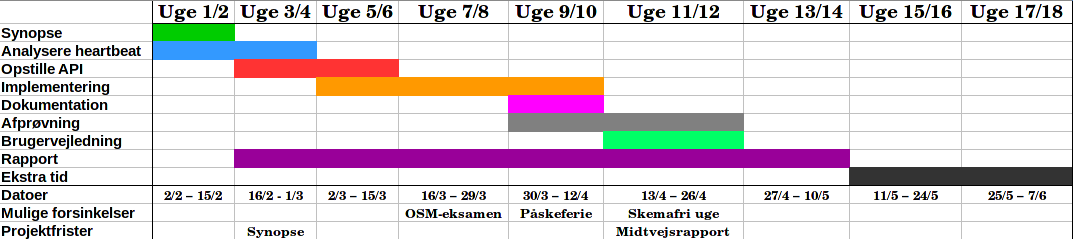
\includegraphics[scale=0.45]{Gantt_diagram_ny.png}

\section*{Evt. metodiske overvejelser, relevant litteratur o.lign}

\url{https://www.usenix.org/system/files/conference/atc14/atc14-paper-ongaro.pdf}  \\
- Beskrivelse af Raft concensus algoritmen - til leader election og logging.
\\[5px]
\url{http://research.microsoft.com/en-us/um/people/lamport/pubs/time-clocks.pdf}  \\
- Beskrivelse af logiske klokker til at sikre konsistens.


\end{document}
